% Copyright (c) 2026 Jonathan Yantis. SPDX-License-Identifier: CC-BY-4.0
\documentclass[10pt,letterpaper]{article}
\usepackage[margin=.70in]{geometry}
\usepackage[T1]{fontenc}
\usepackage{lmodern,microtype,amsmath,amssymb,booktabs,array,xcolor,tikz,listings,enumitem,fancyhdr}
\usetikzlibrary{arrows.meta,positioning}
\usepackage[hidelinks]{hyperref}
\definecolor{ink}{HTML}{24465B}
\definecolor{pale}{HTML}{EDF2F3}
\newcommand{\ns}{\,\mathrm{ns}}
\newcommand{\us}{\,\mu\mathrm{s}}
\newcommand{\src}[1]{\nolinkurl{#1}}
\newcommand{\codepin}{\texttt{b5ecbb0}}
\newcolumntype{L}[1]{>{\raggedright\arraybackslash}p{#1}}
\setlist{nosep,leftmargin=1.4em}
\setlength{\parindent}{0pt}
\setlength{\parskip}{3.6pt}
\setlength{\tabcolsep}{5pt}
\lstset{basicstyle=\ttfamily\small,columns=fullflexible,keepspaces=true,showstringspaces=false,frame=single,rulecolor=\color{ink!35},backgroundcolor=\color{pale},xleftmargin=3pt,xrightmargin=3pt,aboveskip=6pt,belowskip=6pt}
\pagestyle{fancy}\fancyhf{}\fancyhead[L]{\small ESP32-S3 timing implementation notes}\fancyhead[R]{\small DRAFT -- 24 October 2026}\fancyfoot[C]{\thepage}
\setlength{\headheight}{14pt}
\hypersetup{pdftitle={Low-Level Timing on ESP32-S3: Event Capture, Clock Bridges, and Causal Validation},pdfauthor={Jonathan Yantis}}
\begin{document}
\begin{center}
{\LARGE\bfseries Low-Level Timing on ESP32-S3:\\[3pt] Event Capture, Clock Bridges, and Causal Validation}\par
\vspace{7pt}Jonathan Yantis\quad\textit{Independent researcher}\par
24 October 2026\quad Research draft for review; not submitted or peer reviewed
\end{center}
\vspace{-4pt}
\begin{abstract}\noindent
Nanosecond arithmetic is useful only after a timestamp identifies a physical event, its clock domain, and the model available when that event occurred. This implementation paper explains the current PToB ESP32-S3 techniques: a continuous 80 MHz MCPWM capture counter, exact retained-packet association, driver-owned software latches, narrow instruction-RAM clock-read apertures, capture-frozen predictions, dense channel-aware fitting, bounded phase slew, and a separate causal GNSS witness. Four validated Bluetooth-clock projections estimate a programmed transmit time; no physical RF transmit timestamp is claimed. A finite W12 receive observation retained 600/600 relative-PPS samples with 40.795 ns bias-inclusive RMS and 128 ns maximum absolute residual. A downstream witness retained 494 eligible of 600 logged samples and a 372 ns maximum. These are separate, source-relative observations; RF endpoint, reference delay, absolute UTC, transferability and full timing certification remain unqualified. Concrete contracts, equations, pseudocode, failure cases and offline commands are provided for implementers adapting the methods to other systems.
\end{abstract}
\vspace{-4pt}
\section{Start with an event and coordinate contract}
The reference implementation is W12 RC firmware 0.2.10 at \codepin\ [1]. W12 is an ESP32-S3 receiver with an optional BLE100 estimated-TX relay; BLE50 is client-only. Its fine backend is an explicit BLE100 build selection, not a capability of every S3 image. The N30 shares relevant algorithms but has different pin routing and evidence. No W12 GM or HOT source implementation is asserted.

An event record needs more than a scalar time. Retain the raw latch, counter frequency and incarnation, polarity/endpoint convention, event and channel, packet identity, source/root/boot/path scope, and the later time at which the record became available. Physical event time $c_e$ and software availability $c_a$ answer different questions. The former anchors timing; the latter proves causality and latency. Neither a GAP callback nor a successful controller API call supplies an RF event timestamp.

\begin{center}
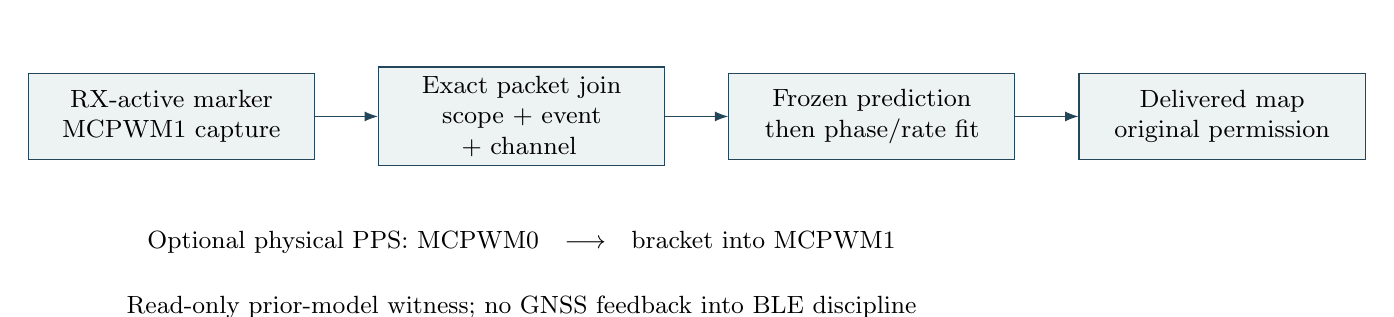
\begin{tikzpicture}[>=Latex,font=\small,box/.style={draw=ink,fill=pale,align=center,minimum height=11mm,text width=34mm},node distance=8mm]
\node[box](edge){RX-active marker\\MCPWM1 capture};
\node[box,right=of edge](join){Exact packet join\\scope + event + channel};
\node[box,right=of join](fit){Frozen prediction\\then phase/rate fit};
\node[box,right=of fit](out){Delivered map\\original permission};
\draw[->,ink](edge)--(join);\draw[->,ink](join)--(fit);\draw[->,ink](fit)--(out);
\node[below=7mm of join,align=center](pps){Optional physical PPS: MCPWM0\quad$\longrightarrow$\quad bracket into MCPWM1};
\node[below=3mm of pps,align=center](shadow){Read-only prior-model witness; no GNSS feedback into BLE discipline};
\end{tikzpicture}
\end{center}
\vspace{-5pt}
\textbf{Three distinct claims.} A 12.5 ns counter tick describes resolution. A signed PPS residual describes agreement with a specified reference and path. A calibrated accuracy bound additionally requires known endpoint, reference, electrical and clock-transfer uncertainty. Keep these quantities distinct in code, plots and acceptance criteria. The architecture above implements useful relative timing while several physical bounds remain unknown.

{\footnotesize Copyright \copyright\ 2026 Jonathan Yantis. Paper and original figure: \href{https://creativecommons.org/licenses/by/4.0/}{CC BY 4.0}. Original code and ordinary repository documentation: MIT. This is a new instructional draft; the separate 22 October empirical paper and its populations are preserved [2].}
\newpage
\section{One continuous counter, with explicit failure modes}
\subsection{Allocate through the driver; latch through a pinned contract}
ESP-IDF documents a dedicated MCPWM capture timer with independent channels. On ESP32-S3 its capture resolution follows the APB source rather than the requested \src{resolution_hz}; query and verify the actual resolution [3]. The W12 fine owner allocates group 1 through the driver, checks 80 MHz, and keeps the timer running through RX windows, packet silence and ordinary model withdrawal. CH0 captures the RX-active marker through GPIO16; CH2 is an enabled software CURRENT latch with no registered ISR. W12 has no fine TX pad. N30 GPIO4/5 assignments must not be copied to W12.

The driver still owns timer/channel lifecycle and power-management state. Low-level code checks the pinned private ABI, enabled state, group/channel, register state and interrupt ownership before using its allocated capture register. A source hash or private-header match establishes compatibility with the reviewed implementation, not physical timing accuracy. Never create a second unowned register reader or let a generic status query change the capture epoch.

\subsection{Extend wraps without using scheduler time as phase}
At 80 MHz a 32-bit counter wraps in 53.6870912 s. The implementation requires a CURRENT observation before half a wrap, 26.8435456 s. For consecutive raw values $r_i$, extend with unsigned modular subtraction:
\[
 d_i=(r_i-r_{i-1})\bmod 2^{32},\qquad C_i=C_{i-1}+d_i,
 \qquad 0\le d_i<2^{31}.
\]
Reject a changed incarnation, backward coarse time, excessive poll gap, nonprogressing timer or integer overflow. Coarse microseconds check liveness and a deliberately loose expected-rate envelope; they never correct the phase of $C$. Poll during packet silence so that a later edge cannot make an ambiguous multi-wrap interval look continuous.

An older captured value $r_e$ is extended relative to a validated CURRENT value, rather than treated as the next current counter. Its modular age $a=(r_i-r_e)\bmod2^{32}$ must fit the retained event-age window (250 ms), the extended range and the fixed origin. This handles an ISR arriving after another read without moving the event to ISR arrival time.

\begin{lstlisting}
current = validate_and_extend(CURRENT_latch, coarse_liveness)
age = uint32(current.raw32 - event.raw32)
require(age <= 80e6 * 0.250 && age <= current.extended)
event80 = current.extended - age
require(event80 >= origin80 && incarnation_matches)
// Only now convert to the consumer's coordinate.
event20 = base20 + round_half_up((event80-origin80-shift80)/4)
\end{lstlisting}

Subtraction, sign and range checks precede conversion. Raw capture stays in 80 MHz units; fine delivered coordinates round to 20 MHz, or 50 ns. A deterministic rounding convention prevents two consumers from assigning different integers to one edge. Do not convert a large UTC epoch to floating point to perform this subtraction.

\subsection{A captured edge still needs an exact packet}
Retain stable controller descriptors and complete packet bytes before the later host callback. The descriptor supplies coarse association, channel and candidate event; it is not silently promoted to a finer RF endpoint. A bounded search requires exactly one rise and one fall in the candidate interval, correct order and incarnation, no pending capture, and no overwritten history. Seal the searched interval; a subsequently discovered late capture invalidates the earlier association. Missing, ambiguous and unsupported cases remain unavailable.

Current PDU191/ext1 traffic uses captured RX-active fall minus 1568 $\mu$s as an \emph{empirical phase convention}. Legacy PDU159/ext0 retains descriptor phase on the same continuous origin. The subtraction is packet-class-specific, not an identified ADDRESS/END event or transferable RF calibration. Preserve both raw marker and convention; a finer latch cannot repair a wrong event definition.
\newpage
\section{Make cross-clock reads into measured apertures}
\subsection{Bracket the operation, not its surrounding bookkeeping}
Independent counters require a bridge. Read the local counter immediately before and after the operation that observes the other clock. If its local latches are $L,H$ and the other reading is $G$, assign the sampled anchor to the midpoint while retaining an enclosure:
\[
 \widehat C(G)=L+\left\lfloor\frac{H-L}{2}\right\rfloor,
 \qquad u_{\rm aperture}\ge\frac{H-L}{2}+u_{\rm rounding}.
\]
This encloses the read operation under its ordering/clock assumptions. It does not measure interconnect, GPIO, synchronizer, detector or RF delay. Retain $L,H,G$, frequency, epoch and method identifier rather than only a midpoint.

The fine GNSS bridge encloses a group 0 CH1 software capture between group 1 CH2 CURRENT captures. The caller holds the GNSS queue critical section so the map callback cannot consume the middle capture before the bracket finishes. Timer ownership and pending-event handling precede the aperture; counter extension, coordinate conversion, statistics and association follow it.

\begin{lstlisting}
validate_driver_owners_and_ROM(); lock_required_owners()
process_pending_physical_edges()       // outside aperture
IRAM_aperture:
  clear_and_confirm(CURRENT_flag)      // finite polling
  trigger_CURRENT(); wait_flag(); L = read_CAPTURE2()
  clear_and_confirm(CURRENT_flag)
  G = read_other_clock_or_trigger_GNSS_capture()
  trigger_CURRENT(); wait_flag(); H = read_CAPTURE2()
unlock_required_owners()
require(aperture_completed && H >= L && within_cycle_budget)
extend_and_convert(L, H, G); publish_map_with_availability()
\end{lstlisting}

Clearing then confirming the flag matters: an old completion flag must not authorize a stale register value. Bound every poll and the total operation. The current implementation uses at most 128 iterations per wait and a 24,000-cycle ceiling at fixed 240 MHz (100 $\mu$s). This is a containment ceiling, not a claimed normal aperture or an RF error bound. Failure refuses the map; it does not fall back to a differently defined clock.

\subsection{Instruction RAM reduces a specific source of variation}
The paired-latch function is \src{noinline} and placed in IRAM. For the Bluetooth bridge the inner operation is one validated ROM Bluetooth-clock read; all validation and coordinate arithmetic stay outside. Inspect the actual ELF and disassembly: source annotations alone do not show what was inlined, where a constant lives, or whether a helper calls flash. Espressif explicitly requires the complete code/data call path of an IRAM-safe handler to remain in internal memory [4]. A small aperture also conserves scarce IRAM and makes the instruction sequence auditable.

Avoid formatting, allocation, locks of uncertain ownership, model fitting and queue traversal inside the bracket. Critical sections serialize a software operation; they cannot remove hardware latency or make two counter domains identical. Keep per-core binding, ROM fingerprint, driver lock order and callback deferral as part of the bridge contract. Measure under the real observer/logging load.

\subsection{Record the achieved width separately from the target}
An earlier W12 0.2.6 paired-latch observation measured 650--750 ns aperture; the later 0.2.7 GNSS read/rounding enclosure was 438--538 ns [5]. These distinct quantities and source versions must not be subtracted from a PPS residual as though either were a known bias. The latter enclosure remains larger than 200 ns despite much smaller observed relative residuals. A narrow interval improves knowledge of the mapping operation; it does not, by itself, certify the whole timing chain.

Compare bridge revisions under frozen workload and event class. Retain failed brackets and width distributions with acceptance coverage. An association anchor and a delivered output estimate have different selection rules.
\newpage
\section{Fit frequency without rewriting delivered history}
\subsection{Freeze the prediction at capture; score before training}
A follow-up correction arrives after its original packet. At the original's capture, save the prediction of the then-delivered clock and a nominal-rate comparison. When the correction becomes available, score those frozen predictions before adding the observation to the fit. Otherwise intervening corrections can train the model on information unavailable at the original edge and make a retrospective residual look causal.

\begin{lstlisting}
on_original(packet, event20):
  saved = {tuple, event20, prior_clock(event20), nominal(event20)}
on_correction(correction, available20):
  require(exact_tuple_match && original_permission_still_valid)
  score_all(saved.prior_prediction - correction.parent_time)
  fit_raw_observation(saved.event20, correction.parent_time)
  publish_new_clock(at_actual_completion20, inherited_deadlines)
\end{lstlisting}

Keep model reference tick, computation completion, activation time and original event time distinct. Retained history must prove that activation preceded a delayed PPS edge. A model merely computed before the callback is insufficient. If insertion overlaps the physical edge or history was evicted, record an activation race or missing model; do not use the newer fit to repair that score.

\subsection{Use repeated channels to separate rate from channel offsets}
The bounded 64-point raw history retains 16 Hz opportunities in the fine backend, about four seconds when reception is complete, rather than decimating to a sparse long history. An independent 32 s expiry still bounds retained points under loss. For local elapsed seconds $x_i$ and parent-minus-nominal residual $y_i$ in ns, center within RF channel $k$:
\[
 \widehat f=\frac{\sum_i(x_i-\overline x_{k(i)})(y_i-\overline y_{k(i)})}
 {\sum_i(x_i-\overline x_{k(i)})^2}\quad[\mathrm{ns/s}=\mathrm{ppb}].
\]
Channel centering prevents a changing channel mix from automatically becoming a frequency change. It does not calibrate per-channel delay. Require sufficient repeated-channel degrees of freedom, at least eight points, at least a two-second span and eight within-channel differences before rate training. Refuse nonfinite or out-of-envelope rates; the numerical rate limit is $\pm50$ ppm. Evaluate fit scatter separately from every frozen causal error, including points not selected for fitting.

Compact history stores bounded local deltas and signed residuals after subtracting an integer origin. Rebase before range exhaustion; refuse overflow instead of truncating a timestamp. Preserve large gross-discontinuity failures and withdraw/reacquire the map rather than absorbing a seconds-scale jump into rate. Authentication identifies the producer; it does not make its timestamp physically continuous.

\subsection{Keep phase, frequency and acceleration separate}
A delivered software clock has an integer anchor, nominal elapsed time, relative rate and remaining phase backlog. Update its parameters while preserving the already delivered value. In fine hold, $|p|<2000$ ns selects 1 ppm slew, or 1000 ns/s; exactly 2000 ns retains bounded acquisition steering. A 1000 ns backlog therefore needs at least one second to disappear. A new rate command cannot instantly erase phase.

Estimate a rate-change guard over at least a one-second baseline; differencing adjacent overlapping fits amplifies quantization and channel noise. The quality projection includes a causal RMS/peak term, quantization, remaining phase, age times rate guard and half age-squared times acceleration guard. It is a conservative software projection with explicit unknowns, not a physical P99. Clip it by original source/model permission. Small fit scatter, an illuminated lock and a long admission lease cannot extend a stale observation's lifetime.
\newpage
\section{Build a causal GNSS witness without creating feedback}
\subsection{Separate physical PPS, UART labels and BLE discipline}
The explicit W12 L76K profile uses UART RX39, hardware PPS41 and supply enable GPIO48 LOW. GNSS is disabled by default; an alias or enclosure does not establish wiring. GNSS observes BLE timing but does not discipline its phase/rate, grant source authority, or create GM/HOT support. Checksum-valid UART activity, fresh valid fix and physical PPS are independent indicators. UART arrival cannot timestamp a PPS edge or independently certify its civil-second association.

Keep two witness models: physical raw80 PPS and its mapped20 counterpart. Their different prediction errors reveal mapping scatter without redefining either as delivered BLE accuracy. Score the next physical PPS using the model already available before that edge, then train with it. Require consecutive sequence numbers, plausible physical intervals, valid mapping and a finite forecast horizon; discontinuity resets history and makes affected scores unavailable.

\subsection{Fit bounded curvature on small integer coordinates}
After 32 consecutive PPS observations, the shadow predictor fits a quadratic to counter residuals. For $j=0,\ldots,31$, let $y_j=C_j-C_0-jF$, $x_j=2j-31$ and $z_j=x_j^2-341$. These centered bases satisfy $\sum x_j=\sum z_j=\sum x_jz_j=0$. With Q16 coefficients,
\[
 b=\frac{\sum x_jy_j}{\sum x_j^2},\quad
 c=\frac{\sum z_jy_j}{\sum z_j^2},\quad
 q=4c,\quad s=2b-124c,\quad a=\overline y-31b+620c.
\]
The relative counter model is $D(t)=a+(F+s)t+qt^2$, with coefficients scaled by $2^{16}$ in the implementation. The guard $|q|/F\le10^{-8}\,\mathrm{s}^{-1}$ limits frequency acceleration $|2q|/F$ to 20 ppb/s. It refuses implausible curvature rather than widening precision authority. Before 32 points, retain explicitly labeled linear warm-up; never relabel those scores as quadratic.

To invert the model for a small counter interval $D$, use the stable root
\[
 t=\frac{2(D-a)}{(F+s)+\sqrt{(F+s)^2+4q(D-a)}}.
\]
This avoids cancellation in the direct quadratic formula when curvature is small. Require a positive discriminant, finite result and bounded interval. Predictions more than three seconds beyond the last PPS are invalid. Integer epochs remain integer; floating point operates on a short relative interval, then split whole seconds and round only the fractional part. The production code also checks input magnitudes and intermediate arithmetic. Recompute range bounds when changing history length, frequency or fixed-point scale.

\subsection{Do not fit civil-time translation into oscillator phase}
The relative clock and signed civil-time offset are separate coordinates. A recently identified T096 producer defect allowed a coarse UART/servo fractional phase into that translation. Source 0.15.169 at \src{1a1fa96} selects a whole-second offset from coarse UTC, leaving the PPS-relative coordinate intact [6]. This chooses the offset only: $\mathrm{UTC}_{ns}=\mathrm{relative}_{ns}+K\,10^9$, $K\in\mathbb Z$. It does not quantize event timestamps; their nanosecond fractions are preserved. The source repair is not fresh hardware validation here; absolute second association remains UNKNOWN.

The earlier W12 population inherited an exact output-minus-relative fraction of $-28{,}835{,}875$ ns. Subtracting it retrospectively is a counterfactual arithmetic check, not a new UTC measurement. A receiver can show tens of ns of relative-PPS agreement while its output carries a millisecond translation error. Verify signed offset, relative epoch, whole-second choice and uncertainty independently. A correct nearest-second calculation cannot establish that the GNSS pulse has been assigned to the correct UTC second by the physical reference chain.
\newpage
\section{Estimated transmit time and honest calibration}
\subsection{Averaging clock projections does not create an RF latch}
The controller hook retains selected payload/publication, event, channel and the programmed half-slot cookie. The worker takes four independently validated Bluetooth/local-clock brackets and projects that same programmed event through each. Decode the 28-bit half-slot count and descending half-microsecond fine field explicitly; handle modular difference before scaling. Reject future, stale, overflowed or inconsistent projections.

For four integer projections $p_i$ in 20 MHz ticks, require all four and $\max p_i-\min p_i\le40$ ticks (2 $\mu$s). Then compute without summing four large epochs:
\[
 m=\min p_i,\qquad \widehat p=m+
 \left\lfloor\frac{\sum_{i=1}^4(p_i-m)+2}{4}\right\rfloor.
\]
The bounded differences make overflow analysis simple. Every valid projection participates; no choice by downstream error and no trimming. Version-4 TX-path diagnostics retain all four. This consistency screen is not an RF uncertainty bound; the four reads can share a systematic mapping error. Keep the narrowest association anchor, if needed, separate from the mean used for the programmed-time estimate.

For LE 1M, 8 preamble bits plus 32 access-address bits take nominally 40 $\mu$s [7]. Project both programmed start and start $+800$ ticks through the same frozen publication model, and use the nominal ADDRESS projection. This repairs a reference convention; controller scheduling-to-preamble delay and TX/RX detector equivalence remain unknown. PHY changes require a new endpoint rule. The model must belong to the bytes actually queued for that publication, not whichever live model is newest when the hook is processed.

\subsection{Treat offsets as scoped empirical parameters}
Current W12 uses a provisional receive adjustment $+7671$ ns on delivered copies, leaving raw oscillator fitting untouched, and a separate relay residual $+4026$ ns beyond nominal ADDRESS. These constants were trained on a particular relative W12/downstream path. Applying the shared values to other units/profiles is an unmeasured transfer, not a calibration certificate. Older aggregate profiles defined as totals from programmed start retain that total meaning; do not add ADDRESS twice. Root/boot/path/profile and source-age applicability must accompany each parameter.

\begin{table}[ht]\centering\small
\caption{Distinct finite observations, all tails retained [5]. RMS includes bias. Values are relative to the named witness, not independently calibrated UTC.}
\begin{tabular}{L{66mm}rrrr}\toprule
Metric and population & Eligible / denominator & Mean ns & RMS ns & Max $|e|$ ns\\\midrule
0.2.7 raw PPS next-edge prediction &600/600&0.568&11.827&101\\
0.2.7 mapped PPS next-edge prediction &600/600&0.760&24.771&85\\
0.2.10 delivered W12 relative PPS &600/600&$-27.122$&40.795&128\\
Downstream delivered relative PPS &494/600 logged&$-52.247$&77.650&372\\
Sampled emitted-TX / received-PPS path &63/120 selected&$-62.889$&104.864&229\\\bottomrule
\end{tabular}
\end{table}

The 0.2.10 W12 population comprises two predeclared 300 s windows: all 600 residuals were strictly below 200 ns and 593 below 100 ns; no final-window refit was used. Downstream had 106 unscorable logged records, mostly activation races, and two eligible residuals at least 200 ns. In the sampled path, 120 selected TX tuples yielded 86 seen RX tuples, 66 follow-up matches and 63 PPS-scored observations; three scored residuals were at least 200 ns. This aggregate received-path comparison does not identify TX delay. The whole timing-certification gate remained FAIL. The earlier 22 October N30 result (657 eligible of 660; 166.590 ns RMS; 1591 ns maximum) is a different population [2], not a pooled benchmark or a W12 baseline.
\newpage
\section{A reproducible implementation and validation sequence}
\begin{enumerate}
\item \textbf{Freeze semantics before tuning.} Name the event, polarity, packet class, clock/boot incarnation, frequency, reference convention, source scope and original expiry. Retain raw latches and software availability. Prove route/resource ownership and power-state behavior; do not infer GNSS capability or RF semantics from a board label.
\item \textbf{Validate arithmetic and lifecycle offline.} Exercise rollover, half-wrap silence, delayed/pending edges, overwritten association windows, changed source, stale/missing model, activation races, stop/drain failure, signed offset, midpoint ties and overflow. Check actual compiled IRAM placement and driver/ROM fingerprints. A successful build validates neither a physical endpoint nor hardware acceptance.
\item \textbf{Characterize counter and bridge first.} Check raw PPS intervals, drift and aperture/enclosure under actual workload. Keep pre-IRAM, post-IRAM, linear and quadratic populations distinct. Count attempts, rejected brackets and unavailable predictions. Compare raw and mapped witness prediction without feeding the witness into BLE fitting.
\item \textbf{Separate training and held-out output.} Prespecify windows and eligibility; freeze offset/profile first. Retain startup, source loss, missing opportunities, invalid records, tails and an end fence. Report signed mean, bias-inclusive RMS, centered spread, maximum, threshold counts and availability denominators. Reusing validation data for tuning changes its status to training.
\item \textbf{Certify the whole claimed endpoint separately.} Independently measure reference PPS/cable/GPIO uncertainty, RF event and detector delays, output electrical timing, UTC second association, transfer across units/profiles, temperature/load behavior and availability. Unknown components remain unknown. A useful implementation or finite relative target can pass while this certification fails.
\end{enumerate}

\subsection{Source, offline checks and reproduction limits}
The local implementation pin is W12 \codepin; publication of current source revisions requires separate authorization. Read \src{firmware/w12/README.md} and \src{docs/w12/build.md}. The capture owner, counter, receiver, corrected clock and TX estimate are in \src{firmware/w12/main/}; the active GNSS predictor is \src{firmware/w12/legacy/ptob_gps_shadow_clock.hpp}. The build guide pins public ESP-IDF v5.5.5 at \src{b774170f}; normal verification does not require a sibling private checkout. These commands open no hardware and use fresh ignored output directories:
\begin{lstlisting}[basicstyle=\ttfamily\footnotesize]
python3 firmware/w12/tools/fine_tests.py --out artifacts/paper-fine-01
python3 firmware/w12/tools/gps_shadow_tests.py --out artifacts/paper-gps-01
# After the documented public SDK setup:
CC=clang CXX=clang++ python3 firmware/w12/tools/g1_host_tests.py \
  --out artifacts/paper-g1-01
python3 tools/verify_s3_low_level_paper.py
tectonic --outdir artifacts/paper-build papers/ptob-esp32s3-low-level-timing.tex
\end{lstlisting}
Supplement [5] exports selected aggregates and source identities, excluding private logs, enrollment and exact device identifiers. Denominator/algebra checks are reproducible; new empirical statistics cannot be recomputed from public per-event rows. Synthetic checks validate algorithms/refusals, not hardware observations. No new deployed result is asserted for repair [6].

\vspace{-3pt}
\begin{thebibliography}{9}\footnotesize\raggedright\setlength{\itemsep}{0pt}\setlength{\parskip}{1pt}
\bibitem{code} J. Yantis. \textit{PToB W12 RC 0.2.10 source}, commit b5ecbb0b13dbab955282327afe16e4d08d24d823, 24 Oct. 2026. Local review source pin; repository: \url{https://github.com/yantisj2/PToB}.
\bibitem{previous} J. Yantis. \textit{Precision Bluetooth Timing on ESP32-S3: Causal Clock Discipline and Hardware Event Capture}, 22 Oct. 2026 draft. PToB, \src{papers/ptob-esp32s3-timing-preprint.pdf}; selected reproducible historical evidence in \src{evidence/s3/2026-10-22-fine/}.
\bibitem{mcpwm} Espressif. \textit{ESP-IDF v5.5.5: MCPWM, capture timer/channels and power management}; \textit{ESP32-S3 Technical Reference Manual}, capture submodule. \href{https://docs.espressif.com/projects/esp-idf/en/v5.5.5/esp32s3/api-reference/peripherals/mcpwm.html}{Official API reference}; \href{https://www.espressif.com/sites/default/files/documentation/esp32-s3_technical_reference_manual_en.pdf}{official TRM}. Accessed 24 Oct. 2026.
\bibitem{iram} Espressif. \textit{ESP-IDF v5.5.5: Interrupt Allocation, IRAM-Safe Interrupt Handlers}. \href{https://docs.espressif.com/projects/esp-idf/en/v5.5.5/esp32s3/api-reference/system/intr_alloc.html}{Official documentation}. Accessed 24 Oct. 2026.
\bibitem{summary} J. Yantis. \textit{Selected aggregate observations for the low-level timing draft}, 24 Oct. 2026, CC BY 4.0. \src{papers/supplements/esp32s3-low-level-2026-10-24.json}. Local research summaries; raw data not included; scope and exclusions retained.
\bibitem{utc} J. Yantis. \textit{T096 0.15.169 UTC-basis source repair}, commit 1a1fa96df54116b877a34cc7fa4445e91c2860f8. Local review source identity; no fresh hardware result asserted here.
\bibitem{ble} Bluetooth SIG. \textit{Core Specification 6.1, Low Energy Controller, Link Layer, packet format}. \href{https://www.bluetooth.com/wp-content/uploads/Files/Specification/HTML/Core-61/out/en/low-energy-controller/link-layer-specification.html}{Official specification}. Accessed 24 Oct. 2026.
\end{thebibliography}
\end{document}
